\newpage
\hypertarget{initialize vis}{}
\subsection{Establishing visual TGGs}
\visHeader

\begin{itemize}

\item[$\blacktriangleright$] From Eclipse, open \texttt{Dict\-ion\-ary.eap} in Enterprise Architect (EA). The project browser should already resemble
Fig.~\ref{ea:mocaTagged}. As you can see, the project is populated with the source \texttt{MocaTree} specification for a generic tree structure in the
\texttt{eMoflon Languages} working set.

\vspace{0.5cm}

\begin{figure}[htpb]
\begin{center}
  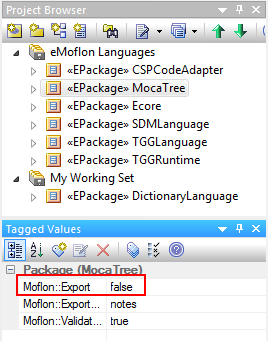
\includegraphics[width=0.4\textwidth]{ea_mocaTaggedValues}
  \caption{Preventing \texttt{MocaTree} from exporting to Eclipse}
  \label{ea:mocaTagged}
\end{center}
\end{figure}

\end{itemize}
\vspace{-0.5cm}
If you inspect the tagged values\footnote{The ``Tagged Values'' window can be opened by going to ``View/Tagged Values'' or by hovering over the \texttt{Tagged
Values} tab immediately to the right of the project browser.} for each language, you'll notice that the \texttt{MocaTree} package has the
\texttt{Moflon::Export} value set to \texttt{false}.
This ensures that the package is \emph{ignored} when exporting. As with all standard metamodels (e.g., Ecore or the SDM metamodel) the \texttt{MocaTree} package in EA should be regarded as read-only, required only in the
EA project so that SDMs can refer to the classes defined in the package. As discussed, the Java code is provided and added automatically by our Eclipse plugin.

\begin{itemize}

\item[$\blacktriangleright$] Go ahead and inspect the \texttt{MocaTree} diagram (Fig.~\ref{ea:mocaTree}). Make sure you understand which attributes and
references each element contains.

\item[$\blacktriangleright$] Despite \texttt{DictionaryLanguage} being contained in a different node than \texttt{MocaTree}, it's clear these two metamodels are
contained within the same project. Therefore, you can start a new TGG by adding a package to \texttt{My Working Set}. Name it
\texttt{Dict\-ion\-ary\-Code\-Adap\-ter}.

\newpage

\begin{figure}[htpb]
  \hspace{-3cm}
  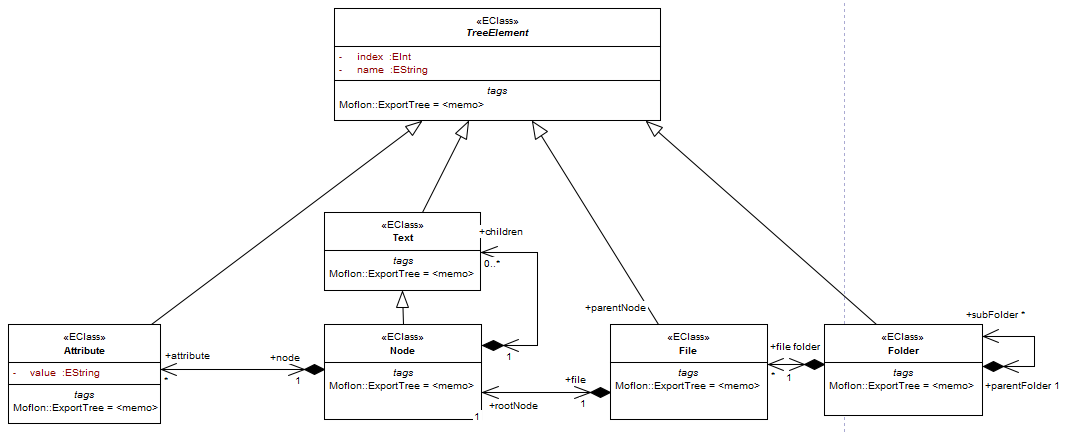
\includegraphics[width=1.5\textwidth]{ea_metamodelMocaTree}
  \caption{The \texttt{MocaTree} metamodel}
  \label{ea:mocaTree}
\end{figure}

\item[$\blacktriangleright$] Select the package and add a new TGG schema diagram as depicted in Fig.~\ref{ea:newTGGDiagram}. In the next dialogue,
set the source project as \texttt{MocaTree}, and the target project as \texttt{Dict\-ion\-ary\-Lang\-uage}.

\begin{figure}[h!]
\begin{center}
  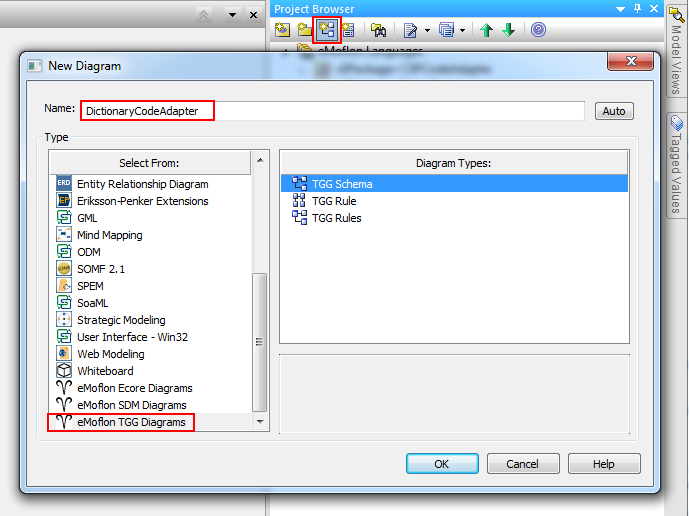
\includegraphics[width=0.9\textwidth]{ea_adapterTGGDiagram}
  \caption{Create a new TGG Diagram}
  \label{ea:newTGGDiagram}
\end{center}
\end{figure}

\end{itemize}

\clearpage

\begin{itemize}

\item[$\blacktriangleright$] To ensure the package exports correctly to Eclipse as a TGG project, add a single correspondence type to your new
diagram (the \texttt{schema}) between \texttt{Folder} and \texttt{Library}. Remember -- you can get the classes by drag-and-dropping each element into the
diagram, then quick-linking a new \texttt{TGG Correspondence Type} between them.\footnote{For details on this correspondence metamodel and how to build types
between classes, refer to Part IV, Section 3.} Your diagram should come to resemble Fig.~\ref{ea:firstCorrType}.

\vspace{0.5cm}

\begin{figure}[htpb]
\begin{center}
  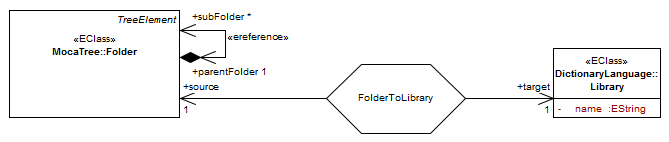
\includegraphics[width=\textwidth]{ea_firstAdapterCorrespondence}
  \caption{The transformation's first correspondence type}
  \label{ea:firstCorrType}
\end{center}
\end{figure}

\item[$\blacktriangleright$] Your project browser should now resemble Fig.~\ref{ea:TGGProjBrow}, where \texttt{Dict\-ion\-ary\-Code\-Adap\-ter} is
explicitly listed as a \texttt{TGGSchemaPackage}.

\vspace{0.5cm}

\begin{figure}[htpb]
\begin{center}
  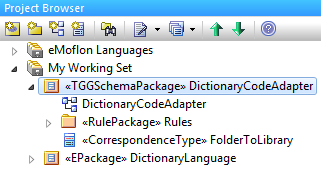
\includegraphics[width=0.5\textwidth]{ea_TGGProjectBrowser}
  \caption{A fully prepared TGG project}
  \label{ea:TGGProjBrow}
\end{center}
\end{figure}

\item[$\blacktriangleright$] Save and validate your file via the eMoflon control panel,\footnote{Actviate via ``Extensions/Add-in Windows''} then switch
back to Eclipse and refresh the package explorer. A new \texttt{Dict\-ion\-ary\-Code\-Adap\-ter} folder should appear under \texttt{My Working Set}; Your TGG setup
is nearly complete!

\jumpSingle{subSec:setupParser}

\end{itemize}
